\documentclass{report}

\documentclass[12pt]{article}
\usepackage{array}
\usepackage{color}
\usepackage{amsthm}
\usepackage{eufrak}
\usepackage{lipsum}
\usepackage{pifont}
\usepackage{yfonts}
\usepackage{amsmath}
\usepackage{amssymb}
\usepackage{ccfonts}
\usepackage{comment} \usepackage{amsfonts}
\usepackage{fancyhdr}
\usepackage{graphicx}
\usepackage{listings}
\usepackage{mathrsfs}
\usepackage{setspace}
\usepackage{textcomp}
\usepackage{blindtext}
\usepackage{enumerate}
\usepackage{microtype}
\usepackage{xfakebold}
\usepackage{kantlipsum}
%\usepackage{draftwatermark}
\usepackage[spanish]{babel}
\usepackage[margin=1.5cm, top=2cm, bottom=2cm]{geometry}
\usepackage[framemethod=tikz]{mdframed}
\usepackage[colorlinks=true,citecolor=blue,linkcolor=red,urlcolor=magenta]{hyperref}

%//////////////////////////////////////////////////////
% Watermark configuration
%//////////////////////////////////////////////////////
%\SetWatermarkScale{4}
%\SetWatermarkColor{black}
%\SetWatermarkLightness{0.95}
%\SetWatermarkText{\texttt{Watermark}}

%//////////////////////////////////////////////////////
% Frame configuration
%//////////////////////////////////////////////////////
\newmdenv[tikzsetting={draw=gray,fill=white,fill opacity=0},backgroundcolor=none]{Frame}

%//////////////////////////////////////////////////////
% Font style configuration
%//////////////////////////////////////////////////////
\renewcommand{\familydefault}{\ttdefault}
\renewcommand{\rmdefault}{tt}

%//////////////////////////////////////////////////////
% Bold configuration
%//////////////////////////////////////////////////////
\newcommand{\fbseries}{\unskip\setBold\aftergroup\unsetBold\aftergroup\ignorespaces}
\makeatletter
\newcommand{\setBoldness}[1]{\def\fake@bold{#1}}
\makeatother

%//////////////////////////////////////////////////////
% Default font configuration
%//////////////////////////////////////////////////////
\DeclareFontFamily{\encodingdefault}{\ttdefault}{%
  \hyphenchar\font=\defaulthyphenchar
  \fontdimen2\font=0.33333em
  \fontdimen3\font=0.16667em
  \fontdimen4\font=0.11111em
  \fontdimen7\font=0.11111em}


%From M275 "Topology" at SJSU
\newcommand{\id}{\mathrm{id}}
\newcommand{\taking}[1]{\xrightarrow{#1}}
\newcommand{\inv}{^{-1}}

%From M170 "Introduction to Graph Theory" at SJSU
\DeclareMathOperator{\diam}{diam}
\DeclareMathOperator{\ord}{ord}
\newcommand{\defeq}{\overset{\mathrm{def}}{=}}

%From the USAMO .tex files
\newcommand{\ts}{\textsuperscript}
\newcommand{\dg}{^\circ}
\newcommand{\ii}{\item}

% % From Math 55 and Math 145 at Harvard
% \newenvironment{subproof}[1][Proof]{%
% \begin{proof}[#1] \renewcommand{\qedsymbol}{$\blacksquare$}}%
% {\end{proof}}

\newcommand{\liff}{\leftrightarrow}
\newcommand{\lthen}{\rightarrow}
\newcommand{\opname}{\operatorname}
\newcommand{\surjto}{\twoheadrightarrow}
\newcommand{\injto}{\hookrightarrow}
\newcommand{\On}{\mathrm{On}} % ordinals
\DeclareMathOperator{\img}{im} % Image
\DeclareMathOperator{\Img}{Im} % Image
\DeclareMathOperator{\coker}{coker} % Cokernel
\DeclareMathOperator{\Coker}{Coker} % Cokernel
\DeclareMathOperator{\Ker}{Ker} % Kernel
\DeclareMathOperator{\rank}{rank}
\DeclareMathOperator{\Spec}{Spec} % spectrum
\DeclareMathOperator{\Tr}{Tr} % trace
\DeclareMathOperator{\pr}{pr} % projection
\DeclareMathOperator{\ext}{ext} % extension
\DeclareMathOperator{\pred}{pred} % predecessor
\DeclareMathOperator{\dom}{dom} % domain
\DeclareMathOperator{\ran}{ran} % range
\DeclareMathOperator{\Hom}{Hom} % homomorphism
\DeclareMathOperator{\Mor}{Mor} % morphisms
\DeclareMathOperator{\End}{End} % endomorphism

\newcommand{\eps}{\epsilon}
\newcommand{\veps}{\varepsilon}
\newcommand{\ol}{\overline}
\newcommand{\ul}{\underline}
\newcommand{\wt}{\widetilde}
\newcommand{\wh}{\widehat}
\newcommand{\vocab}[1]{\textbf{\color{blue} #1}}
\providecommand{\half}{\frac{1}{2}}
\newcommand{\dang}{\measuredangle} %% Directed angle
\newcommand{\ray}[1]{\overrightarrow{#1}}
\newcommand{\seg}[1]{\overline{#1}}
\newcommand{\arc}[1]{\wideparen{#1}}
\DeclareMathOperator{\cis}{cis}
\DeclareMathOperator*{\lcm}{lcm}
\DeclareMathOperator*{\argmin}{arg min}
\DeclareMathOperator*{\argmax}{arg max}
\newcommand{\cycsum}{\sum_{\mathrm{cyc}}}
\newcommand{\symsum}{\sum_{\mathrm{sym}}}
\newcommand{\cycprod}{\prod_{\mathrm{cyc}}}
\newcommand{\symprod}{\prod_{\mathrm{sym}}}
\newcommand{\Qed}{\begin{flushright}\qed\end{flushright}}
\newcommand{\parinn}{\setlength{\parindent}{1cm}}
\newcommand{\parinf}{\setlength{\parindent}{0cm}}
% \newcommand{\norm}{\|\cdot\|}
\newcommand{\inorm}{\norm_{\infty}}
\newcommand{\opensets}{\{V_{\alpha}\}_{\alpha\in I}}
\newcommand{\oset}{V_{\alpha}}
\newcommand{\opset}[1]{V_{\alpha_{#1}}}
\newcommand{\lub}{\text{lub}}
\newcommand{\del}[2]{\frac{\partial #1}{\partial #2}}
\newcommand{\Del}[3]{\frac{\partial^{#1} #2}{\partial^{#1} #3}}
\newcommand{\deld}[2]{\dfrac{\partial #1}{\partial #2}}
\newcommand{\Deld}[3]{\dfrac{\partial^{#1} #2}{\partial^{#1} #3}}
\newcommand{\lm}{\lambda}
\newcommand{\uin}{\mathbin{\rotatebox[origin=c]{90}{$\in$}}}
\newcommand{\usubset}{\mathbin{\rotatebox[origin=c]{90}{$\subset$}}}
\newcommand{\lt}{\left}
\newcommand{\rt}{\right}
\newcommand{\paren}[1]{\left(#1\right)}
\newcommand{\bs}[1]{\boldsymbol{#1}}
\newcommand{\exs}{\exists}
\newcommand{\st}{\strut}
\newcommand{\dps}[1]{\displaystyle{#1}}

\newcommand{\sol}{\setlength{\parindent}{0cm}\textbf{\textit{Solution:}}\setlength{\parindent}{1cm} }
\newcommand{\solve}[1]{\setlength{\parindent}{0cm}\textbf{\textit{Solution: }}\setlength{\parindent}{1cm}#1 \Qed}

% Things Lie
\newcommand{\kb}{\mathfrak b}
\newcommand{\kg}{\mathfrak g}
\newcommand{\kh}{\mathfrak h}
\newcommand{\kn}{\mathfrak n}
\newcommand{\ku}{\mathfrak u}
\newcommand{\kz}{\mathfrak z}
\DeclareMathOperator{\Ext}{Ext} % Ext functor
\DeclareMathOperator{\Tor}{Tor} % Tor functor
\newcommand{\gl}{\opname{\mathfrak{gl}}} % frak gl group
\renewcommand{\sl}{\opname{\mathfrak{sl}}} % frak sl group chktex 6

% More script letters etc.
\newcommand{\SA}{\mathcal A}
\newcommand{\SB}{\mathcal B}
\newcommand{\SC}{\mathcal C}
\newcommand{\SF}{\mathcal F}
\newcommand{\SG}{\mathcal G}
\newcommand{\SH}{\mathcal H}
\newcommand{\OO}{\mathcal O}

\newcommand{\SCA}{\mathscr A}
\newcommand{\SCB}{\mathscr B}
\newcommand{\SCC}{\mathscr C}
\newcommand{\SCD}{\mathscr D}
\newcommand{\SCE}{\mathscr E}
\newcommand{\SCF}{\mathscr F}
\newcommand{\SCG}{\mathscr G}
\newcommand{\SCH}{\mathscr H}

% Mathfrak primes
\newcommand{\km}{\mathfrak m}
\newcommand{\kp}{\mathfrak p}
\newcommand{\kq}{\mathfrak q}

% number sets
\newcommand{\RR}[1][]{\ensuremath{\ifstrempty{#1}{\mathbb{R}}{\mathbb{R}^{#1}}}}
\newcommand{\NN}[1][]{\ensuremath{\ifstrempty{#1}{\mathbb{N}}{\mathbb{N}^{#1}}}}
\newcommand{\ZZ}[1][]{\ensuremath{\ifstrempty{#1}{\mathbb{Z}}{\mathbb{Z}^{#1}}}}
\newcommand{\QQ}[1][]{\ensuremath{\ifstrempty{#1}{\mathbb{Q}}{\mathbb{Q}^{#1}}}}
\newcommand{\CC}[1][]{\ensuremath{\ifstrempty{#1}{\mathbb{C}}{\mathbb{C}^{#1}}}}
\newcommand{\PP}[1][]{\ensuremath{\ifstrempty{#1}{\mathbb{P}}{\mathbb{P}^{#1}}}}
\newcommand{\HH}[1][]{\ensuremath{\ifstrempty{#1}{\mathbb{H}}{\mathbb{H}^{#1}}}}
\newcommand{\FF}[1][]{\ensuremath{\ifstrempty{#1}{\mathbb{F}}{\mathbb{F}^{#1}}}}
% expected value
\newcommand{\EE}{\ensuremath{\mathbb{E}}}
\newcommand{\charin}{\text{ char }}
\DeclareMathOperator{\sign}{sign}
\DeclareMathOperator{\Aut}{Aut}
\DeclareMathOperator{\Inn}{Inn}
\DeclareMathOperator{\Syl}{Syl}
\DeclareMathOperator{\Gal}{Gal}
\DeclareMathOperator{\GL}{GL} % General linear group
\DeclareMathOperator{\SL}{SL} % Special linear group

%---------------------------------------
% BlackBoard Math Fonts :-
%---------------------------------------

%Captital Letters
\newcommand{\bbA}{\mathbb{A}}	\newcommand{\bbB}{\mathbb{B}}
\newcommand{\bbC}{\mathbb{C}}	\newcommand{\bbD}{\mathbb{D}}
\newcommand{\bbE}{\mathbb{E}}	\newcommand{\bbF}{\mathbb{F}}
\newcommand{\bbG}{\mathbb{G}}	\newcommand{\bbH}{\mathbb{H}}
\newcommand{\bbI}{\mathbb{I}}	\newcommand{\bbJ}{\mathbb{J}}
\newcommand{\bbK}{\mathbb{K}}	\newcommand{\bbL}{\mathbb{L}}
\newcommand{\bbM}{\mathbb{M}}	\newcommand{\bbN}{\mathbb{N}}
\newcommand{\bbO}{\mathbb{O}}	\newcommand{\bbP}{\mathbb{P}}
\newcommand{\bbQ}{\mathbb{Q}}	\newcommand{\bbR}{\mathbb{R}}
\newcommand{\bbS}{\mathbb{S}}	\newcommand{\bbT}{\mathbb{T}}
\newcommand{\bbU}{\mathbb{U}}	\newcommand{\bbV}{\mathbb{V}}
\newcommand{\bbW}{\mathbb{W}}	\newcommand{\bbX}{\mathbb{X}}
\newcommand{\bbY}{\mathbb{Y}}	\newcommand{\bbZ}{\mathbb{Z}}

%---------------------------------------
% MathCal Fonts :-
%---------------------------------------

%Captital Letters
\newcommand{\mcA}{\mathcal{A}}	\newcommand{\mcB}{\mathcal{B}}
\newcommand{\mcC}{\mathcal{C}}	\newcommand{\mcD}{\mathcal{D}}
\newcommand{\mcE}{\mathcal{E}}	\newcommand{\mcF}{\mathcal{F}}
\newcommand{\mcG}{\mathcal{G}}	\newcommand{\mcH}{\mathcal{H}}
\newcommand{\mcI}{\mathcal{I}}	\newcommand{\mcJ}{\mathcal{J}}
\newcommand{\mcK}{\mathcal{K}}	\newcommand{\mcL}{\mathcal{L}}
\newcommand{\mcM}{\mathcal{M}}	\newcommand{\mcN}{\mathcal{N}}
\newcommand{\mcO}{\mathcal{O}}	\newcommand{\mcP}{\mathcal{P}}
\newcommand{\mcQ}{\mathcal{Q}}	\newcommand{\mcR}{\mathcal{R}}
\newcommand{\mcS}{\mathcal{S}}	\newcommand{\mcT}{\mathcal{T}}
\newcommand{\mcU}{\mathcal{U}}	\newcommand{\mcV}{\mathcal{V}}
\newcommand{\mcW}{\mathcal{W}}	\newcommand{\mcX}{\mathcal{X}}
\newcommand{\mcY}{\mathcal{Y}}	\newcommand{\mcZ}{\mathcal{Z}}


%---------------------------------------
% Bold Math Fonts :-
%---------------------------------------

%Captital Letters
\newcommand{\bmA}{\boldsymbol{A}}	\newcommand{\bmB}{\boldsymbol{B}}
\newcommand{\bmC}{\boldsymbol{C}}	\newcommand{\bmD}{\boldsymbol{D}}
\newcommand{\bmE}{\boldsymbol{E}}	\newcommand{\bmF}{\boldsymbol{F}}
\newcommand{\bmG}{\boldsymbol{G}}	\newcommand{\bmH}{\boldsymbol{H}}
\newcommand{\bmI}{\boldsymbol{I}}	\newcommand{\bmJ}{\boldsymbol{J}}
\newcommand{\bmK}{\boldsymbol{K}}	\newcommand{\bmL}{\boldsymbol{L}}
\newcommand{\bmM}{\boldsymbol{M}}	\newcommand{\bmN}{\boldsymbol{N}}
\newcommand{\bmO}{\boldsymbol{O}}	\newcommand{\bmP}{\boldsymbol{P}}
\newcommand{\bmQ}{\boldsymbol{Q}}	\newcommand{\bmR}{\boldsymbol{R}}
\newcommand{\bmS}{\boldsymbol{S}}	\newcommand{\bmT}{\boldsymbol{T}}
\newcommand{\bmU}{\boldsymbol{U}}	\newcommand{\bmV}{\boldsymbol{V}}
\newcommand{\bmW}{\boldsymbol{W}}	\newcommand{\bmX}{\boldsymbol{X}}
\newcommand{\bmY}{\boldsymbol{Y}}	\newcommand{\bmZ}{\boldsymbol{Z}}
%Small Letters
\newcommand{\bma}{\boldsymbol{a}}	\newcommand{\bmb}{\boldsymbol{b}}
\newcommand{\bmc}{\boldsymbol{c}}	\newcommand{\bmd}{\boldsymbol{d}}
\newcommand{\bme}{\boldsymbol{e}}	\newcommand{\bmf}{\boldsymbol{f}}
\newcommand{\bmg}{\boldsymbol{g}}	\newcommand{\bmh}{\boldsymbol{h}}
\newcommand{\bmi}{\boldsymbol{i}}	\newcommand{\bmj}{\boldsymbol{j}}
\newcommand{\bmk}{\boldsymbol{k}}	\newcommand{\bml}{\boldsymbol{l}}
\newcommand{\bmm}{\boldsymbol{m}}	\newcommand{\bmn}{\boldsymbol{n}}
\newcommand{\bmo}{\boldsymbol{o}}	\newcommand{\bmp}{\boldsymbol{p}}
\newcommand{\bmq}{\boldsymbol{q}}	\newcommand{\bmr}{\boldsymbol{r}}
\newcommand{\bms}{\boldsymbol{s}}	\newcommand{\bmt}{\boldsymbol{t}}
\newcommand{\bmu}{\boldsymbol{u}}	\newcommand{\bmv}{\boldsymbol{v}}
\newcommand{\bmw}{\boldsymbol{w}}	\newcommand{\bmx}{\boldsymbol{x}}
\newcommand{\bmy}{\boldsymbol{y}}	\newcommand{\bmz}{\boldsymbol{z}}

%---------------------------------------
% Scr Math Fonts :-
%---------------------------------------

\newcommand{\sA}{{\mathscr{A}}}   \newcommand{\sB}{{\mathscr{B}}}
\newcommand{\sC}{{\mathscr{C}}}   \newcommand{\sD}{{\mathscr{D}}}
\newcommand{\sE}{{\mathscr{E}}}   \newcommand{\sF}{{\mathscr{F}}}
\newcommand{\sG}{{\mathscr{G}}}   \newcommand{\sH}{{\mathscr{H}}}
\newcommand{\sI}{{\mathscr{I}}}   \newcommand{\sJ}{{\mathscr{J}}}
\newcommand{\sK}{{\mathscr{K}}}   \newcommand{\sL}{{\mathscr{L}}}
\newcommand{\sM}{{\mathscr{M}}}   \newcommand{\sN}{{\mathscr{N}}}
\newcommand{\sO}{{\mathscr{O}}}   \newcommand{\sP}{{\mathscr{P}}}
\newcommand{\sQ}{{\mathscr{Q}}}   \newcommand{\sR}{{\mathscr{R}}}
\newcommand{\sS}{{\mathscr{S}}}   \newcommand{\sT}{{\mathscr{T}}}
\newcommand{\sU}{{\mathscr{U}}}   \newcommand{\sV}{{\mathscr{V}}}
\newcommand{\sW}{{\mathscr{W}}}   \newcommand{\sX}{{\mathscr{X}}}
\newcommand{\sY}{{\mathscr{Y}}}   \newcommand{\sZ}{{\mathscr{Z}}}


%---------------------------------------
% Math Fraktur Font
%---------------------------------------

%Captital Letters
\newcommand{\mfA}{\mathfrak{A}}	\newcommand{\mfB}{\mathfrak{B}}
\newcommand{\mfC}{\mathfrak{C}}	\newcommand{\mfD}{\mathfrak{D}}
\newcommand{\mfE}{\mathfrak{E}}	\newcommand{\mfF}{\mathfrak{F}}
\newcommand{\mfG}{\mathfrak{G}}	\newcommand{\mfH}{\mathfrak{H}}
\newcommand{\mfI}{\mathfrak{I}}	\newcommand{\mfJ}{\mathfrak{J}}
\newcommand{\mfK}{\mathfrak{K}}	\newcommand{\mfL}{\mathfrak{L}}
\newcommand{\mfM}{\mathfrak{M}}	\newcommand{\mfN}{\mathfrak{N}}
\newcommand{\mfO}{\mathfrak{O}}	\newcommand{\mfP}{\mathfrak{P}}
\newcommand{\mfQ}{\mathfrak{Q}}	\newcommand{\mfR}{\mathfrak{R}}
\newcommand{\mfS}{\mathfrak{S}}	\newcommand{\mfT}{\mathfrak{T}}
\newcommand{\mfU}{\mathfrak{U}}	\newcommand{\mfV}{\mathfrak{V}}
\newcommand{\mfW}{\mathfrak{W}}	\newcommand{\mfX}{\mathfrak{X}}
\newcommand{\mfY}{\mathfrak{Y}}	\newcommand{\mfZ}{\mathfrak{Z}}
%Small Letters
\newcommand{\mfa}{\mathfrak{a}}	\newcommand{\mfb}{\mathfrak{b}}
\newcommand{\mfc}{\mathfrak{c}}	\newcommand{\mfd}{\mathfrak{d}}
\newcommand{\mfe}{\mathfrak{e}}	\newcommand{\mff}{\mathfrak{f}}
\newcommand{\mfg}{\mathfrak{g}}	\newcommand{\mfh}{\mathfrak{h}}
\newcommand{\mfi}{\mathfrak{i}}	\newcommand{\mfj}{\mathfrak{j}}
\newcommand{\mfk}{\mathfrak{k}}	\newcommand{\mfl}{\mathfrak{l}}
\newcommand{\mfm}{\mathfrak{m}}	\newcommand{\mfn}{\mathfrak{n}}
\newcommand{\mfo}{\mathfrak{o}}	\newcommand{\mfp}{\mathfrak{p}}
\newcommand{\mfq}{\mathfrak{q}}	\newcommand{\mfr}{\mathfrak{r}}
\newcommand{\mfs}{\mathfrak{s}}	\newcommand{\mft}{\mathfrak{t}}
\newcommand{\mfu}{\mathfrak{u}}	\newcommand{\mfv}{\mathfrak{v}}
\newcommand{\mfw}{\mathfrak{w}}	\newcommand{\mfx}{\mathfrak{x}}
\newcommand{\mfy}{\mathfrak{y}}	\newcommand{\mfz}{\mathfrak{z}}


\title{\Huge{Ecuaciones Diferenciales}\\Examen Final}
\author{\huge{Sergio Montoya Ramírez}}
\date{}

\begin{document}

\maketitle
\newpage% or \cleardoublepage
% \pdfbookmark[<level>]{<title>}{<dest>}
\pdfbookmark[section]{\contentsname}{toc}
\tableofcontents
\pagebreak

\chapter{Importancia de las hipótesis iniciales en el modelado con ecuaciones diferenciales}

Una de las mayores fortalezas que tienen las ecuaciones diferenciales es su capacidad para modelar gran cantidad de sistemas del mundo real. Desde modelos físicos, como todas las leyes de newton o el ejemplo desarrollado en el capitulo $2.3$ del libro guia, hasta modelos poblacionales o biológicos. Las ecuaciones diferenciales se encuentran en casi cualquier campo de estudio de las ciencias exactas. Sin embargo, como todo modelo este tiene sus limitaciones pues en caso contrario resultaría infinitamente complejo modelar hasta el mas simple de los sistemas. Por lo tanto, las hipótesis iniciales toman un papel muy importante en reducir esta complejidad y lograr resultados suficientemente exactos. En este texto, hablaremos de como las hipótesis iniciales pueden afectar la exactitud de un modelo y daremos un ejemplo de esto para un sistema físico especialmente simple.

Una de las maneras mas fáciles que tenemos para hablar de esto es de manera inductiva. Es decir, hablando desde un caso muy particular y construyendo con ello una imagen mas general. Por lo tanto, iniciemos centrémonos en un sistema concreto. Imagine un resorte pegado a una pared, este se elonga una distancia que llamaremos $x$ (observe la figura \ref{fig:image-resorte-jpeg})

\begin{figure}[h]
  \centering
  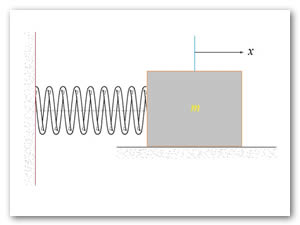
\includegraphics[width=0.6\textwidth]{image/resorte.jpeg}
  \caption{Imagen de referencia para un sistema de resorte elongado con un punto fijo en una pared. Imagen recuperada del articulo de Martin Ortiz Dominguez para la universidad autonoma del estado de hidalgo en el link: https://www.uaeh.edu.mx/scige/boletin/sahagun/n4/a4.html} 
  \label{fig:image-resorte-jpeg}
\end{figure}

Este en si es un sistema relativamente facil y que ya vimos durante el desarrollo de la clase. Incluso dos de nuestros compañeros lo expusieron en un momento determinado. Ahora bien, dado que ya sabemos como funciona esta sistema. Imaginese usted que para desarrollar un modelo decidimos decir que la velocidad durante todo el trayecto es la misma.

\begin{figure}[htpb]
  \centering
  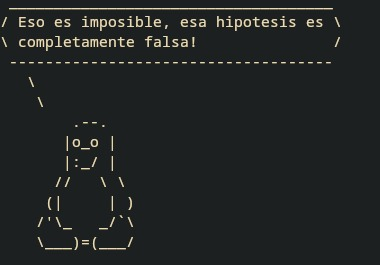
\includegraphics[width=0.4\textwidth]{image/cowsay/tux1.jpeg}
  \caption{Imagen puramente didactica de tux (un pingüino) interpelando que la hipotesis que acabamos de plantear es falsa.}
  \label{fig:image-cowsay-tux1-jpeg}
\end{figure}

Eso lo sabemos tux. Sin embargo, es importante darnos cuenta de que aunque esta hipotesis sea falsa es tan valida (como hipotesis) como cualquier otra. De hecho, en el metodo cientifico el ultimo paso que se hace es comparar los resultados obtenidos con la realidad para asi poder refinar. Por lo tanto, no nos saltemos tantos pasos y asumamos esta hipotesis. Bajo esta hipotesis entonces tenemos
\begin{align*}
  \frac{d x}{dt} = c
.\end{align*}

Ahora bien, para esta ecuación creo que ni siquiera hace falta haber visto el curso de ecuaciones por lo que simplemente dire que se vuelve evidente que 
\begin{align*}
  x = ct + c_2
.\end{align*}

Es decir, la posición va siempre ascendente con respecto al tiempo. Eso eventualmente haria que el resorte se rompiera y todo fallaria. Entonces mostramos que en este caso con una hipotesis falsa nos dirigimos a un resultado absurdo.

Se que el ejemplo que di es especialmente simple y que no veo a nadie que este viendo el curso de ecuaciónes lineales y que no haya podido identificar inmediatamente lo falso del enunciado. Sin embargo, este problema es mucho mas frecuente de lo que nos imaginamos. Siempre que queramos solucionar un problema nos enfrentaremos a escoger una simplificación del estilo. De hecho, solo para aclarar. Incluso en el problema que se trabajo en clase desechabamos en la hipotesis utilizada una realidad física. En este caso hablamos de, por ejemplo, la no fricción de la superficie, ignoramos la fuerza de fluido que aplica el aire en resistencia al movimiento, incluso asumimos que el resorte se encontraba en el vacio por que de caso contrario los resultados variarian. Todo esto sin ni siquiera nombrar el como ignoramos las posibles imperfecciónes de los materiales la precisión de las medidas y el hecho de que la pared sea inamovible. En la solución que dimos ignoramos la tercera ley de newton asumiendo que la pared siendo tan "pesada" no sentiria ningun cambio con la pequeña fuerza que realizo el resorte pero esto no tiene que ser asi. 

Ahora bien, es importante mencionar que todo esto son suposiciones prudentes que hacer para el sistema planteado y que hacen que el problema se enmarque aun mas. Ademas, la mayoria de ellas no aportan demasiado al resultado y la exactitud del modelo es por lo general suficiente. Sin embargo, eh ahi las dos palabras mas importantes exactitud suficiente. La exactitud, se define como que tan cerca dan los resultados de un modelo teorico con los experimentos y suficiente es una medida que se determina en cada caso. En particular en ciencia hablamos de incertidumbre. La incertidumbre es la manera en la que aceptamos que nuestras medidas no pueden ser infinitamente exactos y eso trae en consecuencia que los resultados de un modelo se consideren validos cuando sus resultados esten dentro de la incertidumbre del experimento.

Por lo tanto, las hipotesis son muy importantes a la hora de encontrar un modelo que describa un sistema llevandonos a conclusiones y resultados muy distintos entre si.Sin embargo, las hipotesis se consideraran validas en función de que sus resultados sean suficientemente exactos. 

\chapter{La educación matemática como componente esencial de la formación profesional.}

La matematica es quizas una de las ramas mas importantes de la formación profesional en el area exacta y humana. Esta es una rama del conocimiento que nos permite adquirir conocimientos de manera transversal y tiene su gran fuerza en esto mismo. Es una excelente manera de encontrar verdades y aproximarse al mundo con una herramienta que se ha desarrollado tanto que tiene herramientas para todo el mundo. Las derivadas permitieron a Newton desarrollar una nueva manera de estudiar el movimiento y modelarlo. La topologia permitio a los físicos la creación de una nueva forma de entender el universo. La estadistica hace que los antropologos, sociologos y politologos puedan tener información cuantitativa con la cual tambien pueden analisar fenomenos sociales bajo su contexto. Incluso los filosofos en algun momento lograron integrar logica (Que es una rama que comparten entre ambos) para desarrollar algunas de las pruebas mas hermosas que a traido la filosofia. Por lo tanto, la matematica no es solamente una materia apasionante en si misma y hermosa independiente de todo lo que la rode. Ademas, es la mas potente de todas las herramientas y la manera en la que el ser humano logro entender el mundo que lo rodea y su entorno. No se si como dijo Gauss la matematica es el lenguaje en el que esta escrito el universo. Pero si se que es el lenguaje en el que el humano codifica su saber y aprende del universo. Por lo tanto, la matematica es una de las ramas mas hermosas del conocimiento y esencial para todo el mundo.

\chapter{La continuidad y la derivabilidad como premisas, al abordar el problema de condiciones iniciales}

Durante el desarrollo del curso fuimos viendo en varias ocasiones como una serie de condiciones iniciales y una ecuación diferencial nos podian llevar a un resultado concreto. Ejemplos se vieron muchos, desde los mas sencillos a principio de la clase con ecuaciónes lineales hasta ejemplos mucho mas complejos en sistemas de ecuaciones para el ultimo parcial. Sin embargo, durante todo este desarrollo hablamos de ecuaciónes diferenciales sin preocuparnos por las condiciones que se deben cumplir para que esto sea cierto. En este texto, hablaremos de dos de las condiciones mas importantes que debe cumplir una función para poder ser respuesta de una ecuación diferencial y daremos un ejemplo de por que al ignorar estas condiciones se llega a resultados imposibles.

La primera condición es la continuidad. Iniciaremos por esta dado que esta es necesaria (mas no suficiente) para poder tener la segunda. Ahora bien, ¿Que significa continuidad? una función se define continua en el punto $(x_1,y_1)$ si el limite por izquierda y por derecha tienden a  $f(x_1)$. Esto tiene grandes consecuencias. Una de ellas es que estamos hablando de una noción infinitesimal. Por lo tanto, toda función definida de manera no continua no es derivable en ese punto y en consecuencia no puede ser el resultado de una ecuación diferencial. Un ejemplo de esto es que la función $x$ definida en los naturales no puede ser el resultado de una ecuación diferencial.

La segunda condición es la dervabilidad. Como habiamos dicho antes la derivabilidad es una condición que mas bien se parece a el cumulo de muchas otras. Una de estas es la continuidad, otra es que la función no tenga puntas. En general, que una función sea derivable en el punto $(x_1,y_1)$ significa que 
\begin{align*}
    \lim_{h\to 0} \frac{f\left( x_1+h \right) - f\left( x_1 \right) }{h}
.\end{align*}

existe y tiene un resultado. Esto tambien afecta a los problemas de condiciones iniciales puesto que estas no podrian existir para puntos no derivables de la función. Por ejemplo, una ecuación diferencial cuyo resultado sea $f(x)=|x| + c_1$ no podria tener sus condiciones iniciales en el 0 pues este punto no existe para la derivada y por tanto la ecuación lo eliminaria para poder existir.

Uno de los ejemplos que a mi mas bonitos me parece para mostrar lo problematico que resulta el asumir que podemos derivar ignorando condiciones es mostrar como hacerlo nos lleva de cabeza a absurdos. Imaginemos que tenemos la función $f(x)=x$ definida en los numeros naturales. Sin embargo, dado que estamos en este campo (y saltandonos un poco lo detalles) podemos decir que cada uno de estos $x$ se puede representar como una sumatoria. Esta sumatoria tendria la forma \[
f\left( x \right) = \sum_{n=1}^{x} 1=x
.\] Ahora bien, nada nos detiene para multiplicar esto por $x$ lo cual nos llevaria a definir  $f\left( x \right) $ como \[
f\left( x \right) = \sum_{n=1}^{x} x = x^2
.\] Hasta ahora, no hemos hecho nada mal. Todas las operaciones realizadas son validas para el campo en el que nos encontramos. Sin embargo, asumamos que podemos ignorar las condiciones de derivabilidad y saquemos la derivada de $f(x)$. Esto nos daria:
 \begin{align*}
  \frac{d f(x)}{dx} = \sum_{n=1}^{x} \frac{dx}{dx} = 2x
.\end{align*}

Sin embargo, como pueden notar la derivada de $x$ con respecto a $x$ es $1$ por lo que entonces esto nos queda como
\begin{align*}
  \frac{d f\left( x \right) }{dx} = \sum_{n=1}^{x} 1 = 2x
.\end{align*}

Pero esta definición ya la habiamos visto antes y es $x$. Por lo tanto esto nos lleva a la conclusión de que  $x=2x$ cosa que es completamente absurda para todos los casos. Esto entonces, nos lleva a darnos cuenta que si tenemos una ecuación diferencial cuyo resultado es  $f(x)=x^2+c_1$ podemos estar seguros de que este esta (como minimo) en el campo de los reales. Pues en caso contrario aterrizariamos de cabeza en una contradicción.
\chapter{Las funciones $e^{rt}$, $U\left( t-t_0 \right) $, $\delta\left( t-t_0 \right) $ y $\Gamma\left( s \right) $. Frecuencia de los números irracionales y números complejos en los cálculos, ejemplos.}

Algunos de los casos mas importantes para hablar de ecuaciones diferenciales pasan por conocer algunas de las funciones mas importantes que tenemos para desarrollarlas. En este caso, hablamos de 4 funciones que desarrollaremos cada una por aparte. Por otro lado, tambien tenemos que darnos cuenta de la gran importancia que tienen los numeros irracionales y complejos en las ecuaciones diferenciales. Iniciemos entonces por cada una de estas funciones

\begin{enumerate}
  \item $e^{rt}$ Esta es la función exponencial. Es quizas una de las mas sencillas de entender y es que consiste simplemente en el numero euler (que es un irracional) elevado a $rt$ donde $r$ es una constante y $t$ una variable. Esta es el modelo de solución de las ecuaciones diferenciales de segundo orden homogenas. Es decir ecuaciones de la forma $a y'' + b y' + c y = 0$.
  \item  $U\left( t-t_0) \right) $ Esta es la función escalonada. En verdad una función escalonada no es mas que la función de heaviside a la que le restas un numero para poder mover su centro. Es función en esencia es simplemente \[
  U(t-t_0)= \left\{ \begin{array}{lcc} 1 & si & x \ge 1 \\ \\ 0 & si & x < 0 \end{array} \right.
  .\] que como se puede ver entonces hace que se corra el centro hasta $t_0$. Ahora bien, al concatenar varias de estas funciones escalonadas podemos encontrar cosas sumamente interesantes como por ejemplo la función $\pi\left( x \right) $ la cual es la función que cuenta el numero de numeros primos debajo de $x$. Tambien al multiplicar $U\left( t-t_0 \right) $ con otra función lo que estamos haciendo en esencia es consiguiendo quedarnos unicamente con el lado posterior a $t_0$ de la función lo que tiene amplias aplicaciones en ecuaciones diferenciales.
\item $\delta\left( t-t_0 \right) $ esta es una función delta. La función delta se define como 0 en todo punto exceptuando en $t_0$ en el cual es 1. Por lo tanto, esta función lo que consigue es en esencia eliminar todos los puntos distintos a $t_0$ al multiplicarse por otra función.
\item $\Gamma\left( s \right) $ esta es la función Gamma. La definición en forma de ecuación de esta es compleja. Sin embargo, el objetivo que cumple la misma es relativamente simple. La función gamma desea expandir el concepto de factorial a los complejos. Esto es algo super potente. Por lo general al tener un numero factorial estamos hablando de una productoria desde $1$ hasta  $n$. Sin embargo, esta definición funciona unicamente para numeros naturales. El rol que viene a cumplir la función $\Gamma\left( s \right) $ es poder extender esto a cualquier numero que no sea natural. Tiene gran utilidad por ejemplo a la hora de calcular la transformada de Laplace de $t^{p}$
\end{enumerate}

Por otro lado, la pregunta tambien nos hace pasar por la importancia de los numeros complejos e irracionales y es que a la hora de desarrollar esta materia nos hemos acostumbrado a verlos ampliamente y rara vez nos los cuestionamos. Inicemos por algo que ya dije. Algunas de las ecuaciones iniciales y con las que abrimos el curso tienen su relación con un numero irracional muy importante el numero de Euler. Este numero nos acompaño durante mucho tiempo gracias a sus extrañas caracterizticas como funcion exponencial. Para inicar podemos ver como $\frac{d e^{rx}}{dx}=re^{rx}$. Lo cual da mucho juego puesto que por ello las ecuaciones lineales de segundo orden tienen como respuesta una función exponencial como esta.

Por otro lado, los numeros complejos nos ayudaron muchisimo a la hora de encontrar respuestas. En particular estos siempre se encontraban merodeando y la relación de euler (es decir $e^{it}=\cos\left( t \right) + i\sin\left( t \right) $ nos acompaño durante toda la clase en toda clase de situaciónes. Es de mencionar por ejemplo el importante papel que cumplia a la hora de considerar la solución de sistemas de ecuaciones diferenciales cuando la matriz de representación tenia como eigenvalues numeros complejos.

Por lo tanto, podemos ver que realmente los irracionales y complejos aunque en algun momento de la vida nos pudieron resultar extraños son en verdad bastante frecuentes y utiles para el desarrollo de las ecuaciones diferenciales. 

\chapter{Apreciación personal sobre el desarrollo del curso}

Este fue un curso que inicio de manera interesante. Durante algun tiempo el concepto de ecuación diferencial ya habia reposado en mi cabeza pues lo habia conocido en el curso de Integral. Sin embargo, no sabia realmente con que me iba a enfrentar ni me habia preparado especialmente bien para este curso dado que habia tenido un semestre relativamente complejo en 202301. Sin embargo al llegar comence a entender. Fue un curso en donde muchas cosas del pasado comenzaron a tomar sentido y papel y logre conectar desde las definciones de derivada que tenia desde inicios de carrera hasta las nociones de antiderivada, relación de cambio y modelos. La física de Física I tomo un matiz muy distinto al que tenia hasta ahora. Lo que antes se explicaba con complejos analisis obtusos de dibujos de flechas y calculos que eran extraños resulto entenderse mucho mejor cuando el algebra lineal se combino con las ecuaciones diferenciales y entendi el como estas dos herramientas modelaban muchos sistemas que veia dia a dia. Este fue un curso en donde muchas cosas que tenia en la cabeza tomaron peso y contexto para poder solucionar problemas. Muchas gracias.

\end{document}
